\documentclass{beamer}
%
% Choose how your presentation looks.
%
% For more themes, color themes and font themes, see:
% http://deic.uab.es/~iblanes/beamer_gallery/index_by_theme.html
%
\mode<presentation>
{
  \usetheme{Warsaw}      % or try Darmstadt, Madrid, Warsaw, ...
  \usecolortheme{default} % or try albatross, beaver, crane, ...
  \usefonttheme{default}  % or try serif, structurebold, ...
  \setbeamertemplate{navigation symbols}{}
  \setbeamertemplate{caption}[numbered]
} 

\usepackage[english]{babel}
\usepackage[utf8]{inputenc}
\usepackage[ELEC]{aaltologo}
\usepackage{verbatim}


\title[SFO protocol]{Sensor Fusion and Optimization: Protocol Specification}
\author{Riku Lääkkölä \and Tero Marttila \and Tero Paloheimo}
\institute{Aalto ELEC}
\date{4.2.2014}
\logo{\AaltoLogoRandomSmall{0.3}}

\begin{document}

\begin{frame}
  \titlepage
\end{frame}

\begin{frame}{Introduction}
\begin{itemize}
	\item Unreliable ordered delivery
    \item Idempotent state updates
\end{itemize}
\end{frame}

\begin{frame}{Encoding}
\begin{itemize}
	\item Fixed-length binary header
    \item Variable-length JSON payload
\end{itemize}
\end{frame}

\begin{frame}{Header}
\begin{figure}
	%\centering
	{\scriptsize\verbatiminput{headerfmt.txt}}
	\caption{Message format}
	\label{fig:header}
\end{figure}
\end{frame}

\begin{frame}{Messages}
\begin{table}
	%\centering
	\caption{Message variants}
    %\begin{tabular}{|l|l|l|l|l|l|l|}
\hline
						& 							& \multicolumn{4}{c|}{Header field value} &	\\
Message					& Direction 				& N	& T	& Ack-seq				& Seq	&	Payload \\
\hline
subscribe-query			& Cl $\rightharpoonup$ S		& 1	& 0 	& 0						& 0	&	\\
\hline
subscribe-queryresponse	& Cl $\leftharpoondown$ S	& 1	& 0		& 0						& 0	&	x \\
\hline
subscribe-request		& Cl $\rightharpoonup$ S		& 1	& 0		& 0						& \emph{Cl-sseq++} &
	x \\
\hline
subscribe-response		& Cl $\leftharpoondown$ S	& 1	& 0		& \emph{Cl-sseq}	& \emph{S-sseq++} &	
	x \\
\hline
subscribe-update		& Cl $\leftharpoonup$ S		& 1	& 0		& 0						& \emph{S-sseq++} &
	x \\
\hline
subscribe-ack			& Cl $\rightharpoondown$ S	& 1	& 0		& \emph{S-sseq}	& 0	&	\\
\hline
publish					& Cl $\leftharpoonup$ S		& 1	& 1		& 0						& \emph{S-pseq++} &
	x \\
\hline
publish	(/w NoAck)      & Cl $\leftharpoonup$ S		& 0	& 1		& 0						& \emph{S-pseq++} &
	x \\
\hline
publish-ack				& Cl $\rightharpoondown$ S	& 1	& 1		& \emph{S-pseq}			& \emph{nrecvd}	&	\\
\hline
teardown		      & Cl $\rightharpoonup$ S		& 1	& 2		& 0			& 0	& \\
\hline
teardown-ack		& Cl $\leftharpoondown$ S 		& 1 & 2		& 0			& 0 &	\\
			
\hline
\end{tabular}
	\label{tbl:messages}
\end{table}
\end{frame}

\begin{frame}{Sensor List}
\begin{description}
	\item[subscribe-query]
    \item[subscribe-response]
\end{description}
\end{frame}

\begin{frame}{Subscribe}
\begin{description}
	\item[subscribe-request]
    \item[subscribe-response]
\end{description}
\end{frame}

\begin{frame}{Subscribe example}
\begin{figure}
	%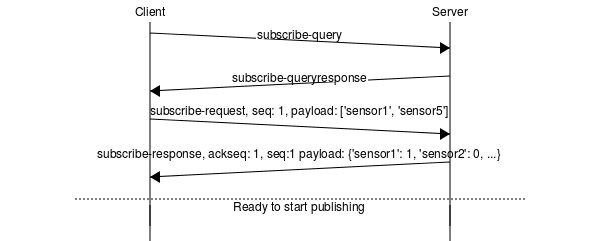
\includegraphics[width=\textwidth]{subscribe_normal.png}
\end{figure}
\end{frame}

\begin{frame}{Subscribe packet loss example}
\begin{figure}
	%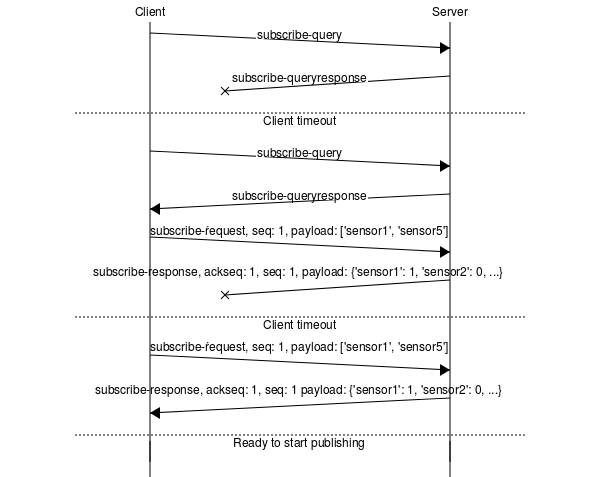
\includegraphics[width=\textwidth]{subscribe_lost.png}
\end{figure}
\end{frame}

\begin{frame}{Publish}
\begin{description}
	\item[publish]
    \item[publish-ack]
\end{description}
\end{frame}

\begin{frame}{Publish example}
\begin{figure}
	%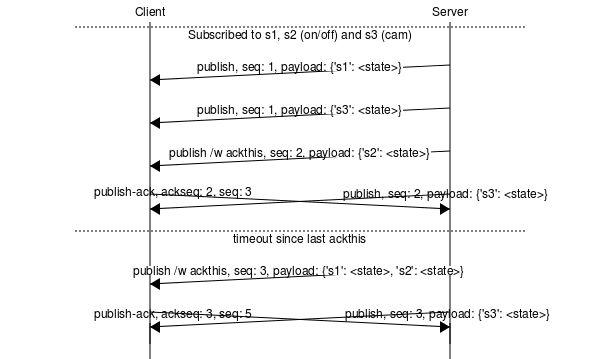
\includegraphics[width=\textwidth]{publish_normal.png}
\end{figure}
\end{frame}

\begin{frame}{Teardown}
\begin{description}
	\item[teardown]
    \item[teardown-ack]
\end{description}
\end{frame}

\begin{frame}{Limitations}
\begin{itemize}
	\item Subscription message size grows linearly with sensor count
    \item No provision for retransmitting lost camera data
\end{itemize}
\end{frame}

\begin{frame}{Conclusion}
\begin{itemize}
	\item Optimize subscribe for reliability
    \item Keepalive timeouts for detecting dropped clients
    \item Handle dropped \textbf{teardown-ack}s
\end{itemize}
\end{frame}

\end{document}
